\documentclass[a4paper,12pt,hidelinks]{report}

%%Pacchetti utili anche se non necessari

\usepackage{amsfonts}
\usepackage{amsmath}
\usepackage{latexsym}
\usepackage{tabularx}
\usepackage[italian]{babel}
\usepackage[bookmarks=true]{hyperref}
\usepackage{url}
% \usepackage{subfigure}
\usepackage{epstopdf}
\usepackage[utf8]{inputenc}
% \usepackage[utf8x]{inputenc}
\usepackage{listings}
\usepackage{graphicx}
\usepackage{color}


%-------------------------------------------

% \title{Progettazione sito web\\ ''B\&B La Vecchia Posta''}
% \author{Daniele Di Pompeo \\mat. 226766}
% \annoaccademico{2013-2014}
\begin{document}
  \begin{titlepage}
    \begin{center}
    % Upper part of the page
      
\includegraphics[width=0.5\textwidth,keepaspectratio=true]{../img/logo}\\[1cm]    
      \textsc{\LARGE Verifiche stile}\\[0.6cm]
      \textsc{\LARGE  progetto del sito:\\[0.5cm] ``B\&B La Vecchia Posta''}\\ [2.0cm]

    % Author and supervisor
      \begin{minipage}{0.8\textwidth}
	\begin{flushleft} \large
	  \emph{Autore:} Daniele Di Pompeo \\[0.5cm]
	  \emph{Versione documento: 1.0}\\[0.5cm]
	  \emph{Data emissione del documento: \today}\\[0.5cm]
	\end{flushleft}
      \end{minipage}
    \end{center}
  \end{titlepage}

% \tableofcontents
 
\begin{abstract}
Lo scopo del seguente documento è convalidare le scelte di scelte progettate differentemente. 
La prima parte descriverà la qualità grafica, successivamente verrà posta
l'attenzione per la compatibilità tra browser e in ultimo ma non meno importante si porrà l'attenzione sul rispetto dei requisiti per l'accessibilità per persone diversamente
abili.
\end{abstract}

\section*{Qualità della grafica}
Per valutare gli aspetti grafici si sono seguite le linee guide più classiche.
Gli oggetti cliccabili risultano essere tutti distinguibili avendo utilizzato un effetto di transizione grafica con attenzione all'utilizzo del cursore pointer del mouse.
\par Le varie sezioni del sito risultano essere identificabili grazie ad un effetto grafico sugli elementi del menu (aumento del weight del font) e grazie all'utilizzo 
del breadcrump.
\par Sono stati inseriti 
\par Le varie sezioni del sito mantengono la stessa disposizione degli elementi non causando ``labirintite'' all'utente.

\subsection*{Colori}

\begin{figure}[h!]%
    
\includegraphics[width=0.4\textwidth,keepaspectratio=true]{../img/logo}
    \centering
    \caption{Layout colori: logo}%
    \label{fig:logo}%
\end{figure}


\begin{figure}[h!]%
    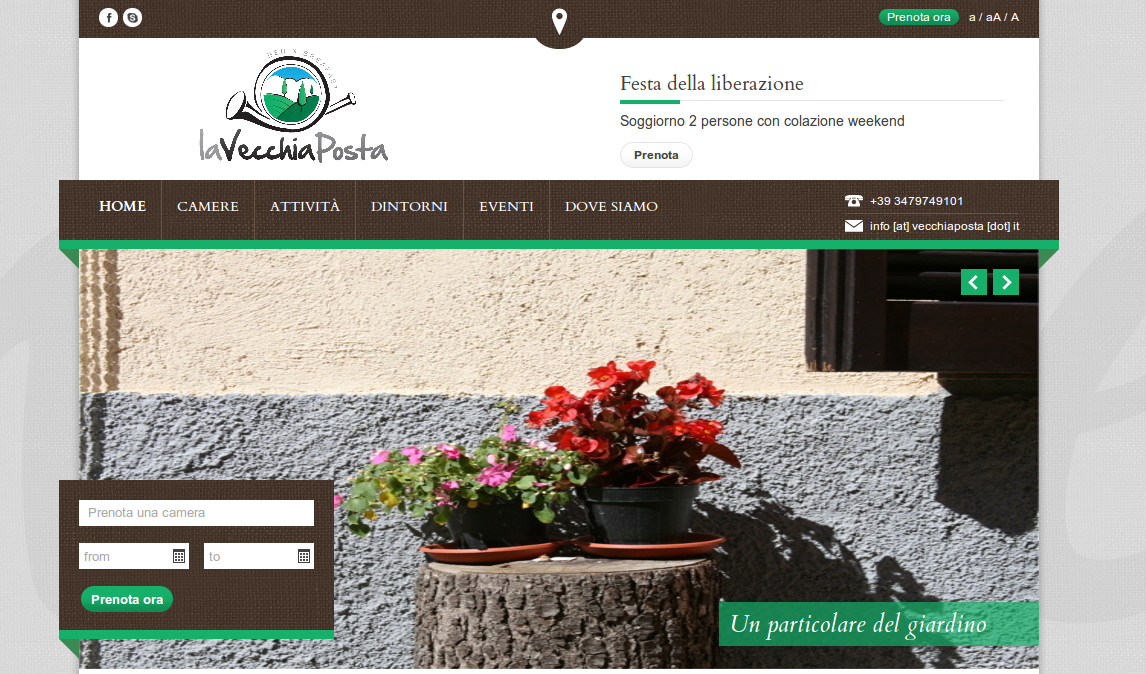
\includegraphics[width=0.9\textwidth,keepaspectratio=true]{../img/layoutHome}
    \centering
    \caption{Layout colori: header e slider}%
    \label{fig:header_slider}%
\end{figure}


\newpage
\subsection*{Dimensione componenti}


\section*{Tipografia}

\end{document}          